% This is "sig-alternate.tex" V2.1 April 2013
% This file should be compiled with V2.5 of "sig-alternate.cls" May 2012
%
% This example file demonstrates the use of the 'sig-alternate.cls'
% V2.5 LaTeX2e document class file. It is for those submitting
% articles to ACM Conference Proceedings WHO DO NOT WISH TO
% STRICTLY ADHERE TO THE SIGS (PUBS-BOARD-ENDORSED) STYLE.
% The 'sig-alternate.cls' file will produce a similar-looking,
% albeit, 'tighter' paper resulting in, invariably, fewer pages.
%
% ----------------------------------------------------------------------------------------------------------------
% This .tex file (and associated .cls V2.5) produces:
%       1) The Permission Statement
%       2) The Conference (location) Info information
%       3) The Copyright Line with ACM data
%       4) NO page numbers
%
% as against the acm_proc_article-sp.cls file which
% DOES NOT produce 1) thru' 3) above.
%
% Using 'sig-alternate.cls' you have control, however, from within
% the source .tex file, over both the CopyrightYear
% (defaulted to 200X) and the ACM Copyright Data
% (defaulted to X-XXXXX-XX-X/XX/XX).
% e.g.
% \CopyrightYear{2007} will cause 2007 to appear in the copyright line.
% \crdata{0-12345-67-8/90/12} will cause 0-12345-67-8/90/12 to appear in the copyright line.
%
% ---------------------------------------------------------------------------------------------------------------
% This .tex source is an example which *does* use
% the .bib file (from which the .bbl file % is produced).
% REMEMBER HOWEVER: After having produced the .bbl file,
% and prior to final submission, you *NEED* to 'insert'
% your .bbl file into your source .tex file so as to provide
% ONE 'self-contained' source file.
%
% ================= IF YOU HAVE QUESTIONS =======================
% Questions regarding the SIGS styles, SIGS policies and
% procedures, Conferences etc. should be sent to
% Adrienne Griscti (griscti@acm.org)
%
% Technical questions _only_ to
% Gerald Murray (murray@hq.acm.org)
% ===============================================================
%
% For tracking purposes - this is V2.0 - May 2012

\documentclass{sig-alternate-05-2015}
\usepackage{url}
\usepackage{epsfig}
\usepackage{makeidx}         % allows index generation
\usepackage{graphicx}        % standard LaTeX graphics tool
                             % when including figure files
\usepackage{multicol}        % used for the two-column index
\usepackage[bottom]{footmisc}% places footnotes at page bottom
\usepackage{float}           % H para posicionar figuras
\usepackage{booktabs}
\begin{document}

% Copyright
\setcopyright{acmcopyright}
%\setcopyright{acmlicensed}
%\setcopyright{rightsretained}
%\setcopyright{usgov}
%\setcopyright{usgovmixed}
%\setcopyright{cagov}
%\setcopyright{cagovmixed}


% DOI
\doi{10.475/123_4}

% ISBN
\isbn{123-4567-24-567/08/06}

%Conference
\conferenceinfo{MSR '16}{May 14-15, 2016, Austin, Texas, USA}

\acmPrice{\$15.00}

%
% --- Author Metadata here ---
\conferenceinfo{MSR}{'16 Austin, Texas USA}
%\CopyrightYear{2007} % Allows default copyright year (20XX) to be over-ridden - IF NEED BE.
%\crdata{0-12345-67-8/90/01}  % Allows default copyright data (0-89791-88-6/97/05) to be over-ridden - IF NEED BE.
% --- End of Author Metadata ---

\title{Who introduced the bug? The importance of the previous commit}
%\subtitle{[Extended Abstract]
%\titlenote{A full version of this paper is available as
%\textit{Author's Guide to Preparing ACM SIG Proceedings Using
%\LaTeX$2_\epsilon$\ and BibTeX} at
%\texttt{www.acm.org/eaddress.htm}}}
%
% You need the command \numberofauthors to handle the 'placement
% and alignment' of the authors beneath the title.
%
% For aesthetic reasons, we recommend 'three authors at a time'
% i.e. three 'name/affiliation blocks' be placed beneath the title.
%
% NOTE: You are NOT restricted in how many 'rows' of
% "name/affiliations" may appear. We just ask that you restrict
% the number of 'columns' to three.
%
% Because of the available 'opening page real-estate'
% we ask you to refrain from putting more than six authors
% (two rows with three columns) beneath the article title.
% More than six makes the first-page appear very cluttered indeed.
%
% Use the \alignauthor commands to handle the names
% and affiliations for an 'aesthetic maximum' of six authors.
% Add names, affiliations, addresses for
% the seventh etc. author(s) as the argument for the
% \additionalauthors command.
% These 'additional authors' will be output/set for you
% without further effort on your part as the last section in
% the body of your article BEFORE References or any Appendices.

\numberofauthors{3} %  in this sample file, there are a *total*
% of EIGHT authors. SIX appear on the 'first-page' (for formatting
% reasons) and the remaining two appear in the \additionalauthors section.
%
\author{
% You can go ahead and credit any number of authors here,
% e.g. one 'row of three' or two rows (consisting of one row of three
% and a second row of one, two or three).
%
% The command \alignauthor (no curly braces needed) should
% precede each author name, affiliation/snail-mail address and
% e-mail address. Additionally, tag each line of
% affiliation/address with \affaddr, and tag the
% e-mail address with \email.
%
% 1st. author
\alignauthor
Gema Rodriguez\\
       \affaddr{University King Juan Carlos}\\
       %\affaddr{1932 Wallamaloo Lane}\\
       \affaddr{Madrid, Spain}\\
       \email{gerope@libresoft.es}
% 2nd. author
\alignauthor
Jesus M. Gonzalez-Barahon\\
      \affaddr{University King Juan Carlos}\\
       %\affaddr{1932 Wallamaloo Lane}\\
       \affaddr{Madrid, Spain}\\
       \email{jgb@gsyc.es}
% 3rd. author
\alignauthor Gregorio Robles\\
       \affaddr{University King Juan Carlos}\\
       %\affaddr{1932 Wallamaloo Lane}\\
       \affaddr{Madrid, Spain}\\
       \email{grex@gsyc.es}
\and  % use '\and' if you need 'another row' of author names
}
% There's nothing stopping you putting the seventh, eighth, etc.
% author on the opening page (as the 'third row') but we ask,
% for aesthetic reasons that you place these 'additional authors'
% in the \additional authors block, viz.
%\additionalauthors{Additional authors: John Smith (The Th{\o}rv{\"a}ld Group,
%email: {\texttt{jsmith@affiliation.org}}) and Julius P.~Kumquat
%(The Kumquat Consortium, email: {\texttt{jpkumquat@consortium.net}}).}
\date{29 January 2016}
% Just remember to make sure that the TOTAL number of authors
% is the number that will appear on the first page PLUS the
% number that will appear in the \additionalauthors section.

\maketitle
\begin{abstract}
To fix a bug in a certain software product, some parts of its source code are modified. At first glance, it could seem reasonable that the fixed bug was introduced by the previous modification of those same parts of the source code (the previous commit). In fact, many studies on bug seeding start with this assumption. However, there is little empirical evidence supporting this assumption, and there are reasons to suppose that in some cases the bug was introduced by other actions, such as an older modification, or a change in called APIs.

This paper tries to shed some light on this area, by analyzing the relationship of bug fixes with their previous commits. To this end, we conducted an observational study on bug reports, their fixes, and their correspoonding previous commits for OpenStack. Our results show that the mentioned asumption does not hold for a large fraction of the analyzed bugs, which were not introduced by their previous commit.
\end{abstract}


%
% The code below should be generated by the tool at
% http://dl.acm.org/ccs.cfm
% Please copy and paste the code instead of the example below.
%
%\begin{CCSXML}
%<ccs2012>
% <concept>
%  <concept_id>10010520.10010553.10010562</concept_id>
%  <concept_desc>Computer systems organization~Embedded systems</concept_desc>
%  <concept_significance>500</concept_significance>
% </concept>
% <concept>
%  <concept_id>10010520.10010575.10010755</concept_id>
%  <concept_desc>Computer systems organization~Redundancy</concept_desc>
%  <concept_significance>300</concept_significance>
% </concept>
% <concept>
%  <concept_id>10010520.10010553.10010554</concept_id>
%  <concept_desc>Computer systems organization~Robotics</concept_desc>
%  <concept_significance>100</concept_significance>
% </concept>
% <concept>
%  <concept_id>10003033.10003083.10003095</concept_id>
%  <concept_desc>Networks~Network reliability</concept_desc>
%  <concept_significance>100</concept_significance>
% </concept>
%</ccs2012>
%\end{CCSXML}

%\ccsdesc[500]{Computer systems organization~Embedded systems}
%\ccsdesc[300]{Computer systems organization~Redundancy}
%\ccsdesc{Computer systems organization~Robotics}
%\ccsdesc[100]{Networks~Network reliability}


%
% End generated code
%

%
%  Use this command to print the description
%
%\printccsdesc

% We no longer use \terms command
%\terms{Theory}

\keywords{Bug introduction, bug seeding, SZZ algoritm, previous commit}

\section{Introduction}
\label{sec:introduction}
%How to plan to apply the knowledge in a way that can benefit software engineers.
%What are the anticipated contributions of the work?  How will you evaluate them to demonstrate usefulness?

%Many efforts on how and why bugs are introduced in the software source code are underway in the software engineering research community. Software source code is affected by many changes, many of them due to failure of the software because of emergent bugs. Concepts such as bug seeding help us to find how and where a bug was inserted in the source code, and which is the responsible line for a bug~\cite{zimmermann2005mining}.

%The current body of knowledge presents a wide collection of tools~\cite{kim2006automatic,fejzer2015supporting} that analyzes the code, and suggest where a potential bug can be found. Other publications describe how to find an error in the source code~\cite{yin2011fixes,zimmermann2006mining}. 

%These articles are based on an implicit assumption: that the line that contains the error was caused by the immediately previous commit as in~\cite{kim2008classifying}, where the authors introduce a new technique to classify changes into two main categories, buggy or clean. In fact they assume the last commit contains the line with the bug. Other authors~\cite{sliwerski2005changes} do not even mention who is the responsible, because they (implicitly) assume the fixed bugs were introduced in the previous commits.

We refer to such \textit{previous commit} that the commit immediately before the bug fix.

%While performing research on the topic, we did not find any empirical evidence that supported this assumption, so we decided to investigate its validity in the case of a large project, such as the OpenStack free/open source cloud computing infrastructure software.

%In order to investigate if this assumption is valid, we formulate following research questions:
In this paper, we attempt to address the following research question regarding who introduced the bug in the source code.
\begin{itemize}
    \item RQ1 : How can tickets which are bug reports be differentiated from those that are not?
    \item RQ2:  How often is the bug caused in the previous commit?
\end{itemize}

The remainder of this paper is structured as follows. First, we present the motivations that support our study,  explaining the current problem in section~\ref{sec:assumption}. Then, Section~\ref{sec:caseStudy} describes our empirical study in an open source project such as OpenStack, followed by the results in Section~\ref{sec:results}. Section~\ref{sec:discussion} discusses potential applications and improvements of our approach. Section~\ref{sec:threats} reports threats to validity. Finally, Section~\ref{sec:related} presenst the actual body of knowdeadge about who caused the bug and Section~\ref{sec:conclusions} concludes the article.

\section{The Current Assumption}
\label{sec:assumption}

- Problem of missclassification\\
- Problem of little empirical evidence about the hypotesis.\\

\section{The Case of Study}
\label{sec:caseStudy}

OpenStack was particularly of interest because of its continuously evolving due to its very active community. Although its short life, only five years, more than 5 thousand of resarchers and more than 233 thousand of commits with more than 2 Million of lines of code have contributed in the development of the project \footnote{\url{http://activity.openstack.org/dash/browser/}}. Futhermore, all history is saved and available in a version control system, being able to access to its issue tracking system \footnote{\url{https://launchpad.net/openstack}} and the source code review \footnote{\url{https://review.openstack.org/}}

OpenStack is composed by 10 projects, but we only focused in the four more actives in the 2015, Nova, Cinder, Neutron and Horizon as we can see in table \ref{tab:OpenStack}
\begin{table}[htb]
\centering
%\begin{center} {\footnotesize
\caption{ Commits per Project in OpenStack}
\label{tab:OpenStack}
\begin{tabular}{lll}
\toprule[0.3mm]%{\smallskip}
  & All History \kern 1pc & Last Year (2015) \\\hline
Nova    \kern 1pc & (184) 55\% & (115) 34\%  \\
Fuel    \kern 1pc & (188) 76\% & (54) 22 \%  \\
Netron  \kern 1pc & (188) 56\% & (116) 35\% \\
Openstack-manuals \kern 1pc & (184) 55\% & (115) 34\%  \\
Horizon \kern 1pc & (188) 76\% & (54) 22 \%  \\
Cinder  \kern 1pc & (188) 56\% & (116) 35\% \\
Keystone\kern 1pc & (184) 55\% & (115) 34\%  \\
Heat    \kern 1pc & (188) 76\% & (54) 22 \%  \\
Glance  \kern 1pc & (188) 56\% & (116) 35\% \\
Tempest \kern 1pc & (188) 56\% & (116) 35\% \\
\bottomrule[0.3mm]
\end{tabular} %}
%\end{center}
\end{table}

In this four projects we analized the relationship of bug fixes with their previous commits. In order to that, we extract a total of 459 tickets from this projects, in which we should be sure that the bug fixes come from a bug report, because two of five issues are misclassified \cite{herzig2013s} and this should cause bias in our final results.

\subsection{Fist Stage: The Filtering}
\label{sec:firstStage}
At this stage and with a tool's support developed to classify bug reports from other issues we distinguished the real bug reports in which afterwards analyzed the relation of the bug fixes with their previous commit.

We use the tool to analyze 459 randomly tickets from the four principal repositories in OpenStack. This tickets could be tagged as either "Fix Commited" or "Fix Released", to be able to localize the patch implemented into de source code in the version repository. They are generally tracked in Launchpad \texttt{Nova},\texttt{Cinder},\texttt{Horizon} and \texttt{Neutron}\footnote{\url{https://bugs.launchpad.net/NameOfRepository}}

Each ticket has an id unique in Launchpad, which will be referred as \textit{n\_ticket}. Given its id, all information about the bug is publicly available in the issues tracking system\footnote{\url{https://bugs.launchpad.net/cinder/+bug/n_ticket}}. OpenStack uses Gerrit as code review system to see the evolution of each bug report\footnote{\url{https://review.openstack.org/ }}. Specifically we found the code review for each \textit{'n\_ticket'}\footnote{\url{https://review.openstack.org/#/c/n_review}}, where \textit{'n\_review'} is the review unique id for each \textit{'n\_ticket'}. In the code review all the information about the patchset that fixed the bug is shown.

The parameters analyzed for each ticket, to distinguish bug reports from others, were the title and the description of the issue report and the description of the fix commit. Also, the code changes if neither the descriptions and the comments clarified the underlying ticket. Each ticket was then categorized into one of three following groups.
\begin{enumerate}
  \item The ticket describes a bug report.
  \item The ticket describes a feature, an optimization code, changes in test files or other not bug reports.
  \item The ticket presents a vague description and cannot be classified without doubts.
\end{enumerate}

Henceforth, we will refer to Group 1 as \textit{Bug Report}, Group 2 as \textit{Not Bug Report} and Group 3 as \textit{Undecided}.

The researchers found main differences to extract data or to classify. In case of disagreement about the ticket classification among researchers, four criteria were used:
\begin{itemize}
    \item When there are only test files in the ticket, we classified it as note being a bug report. Test files in a ticket will not be analyzed, they are indispensables and used as testing method to determine whether the code is fit for use. Sometimes the developers inserted the bug only in the test files, in these cases the ticket was not considered as bug report because the software works as expected only failed the test.
    \item When the title described a new feature, our criteria indicated that it was not a bug report. New features are not considered bug reports, because there is no failure. The optimization, deletion of a dead code or the implementation of new characteristics are included in this criteria. 
    \item When the title described the program as not working as expected, our criteria indicated that it was a bug report. Sometimes the bug is not in a main function which prevents \texttt{Cinder} from working, because a developer has considered it an important bug, although not relatively important. But it is not working as he/she expected. 
    \item When the title described that updates were required, our criteria indicated that it was a bug report. We consider all tickets that require updating as bug reports, because updating a software hints to the software not operating as expected. 
\end{itemize}

Sometimes we were unable to answer all the questions due to having insufficient data or because of the complexity of the issue. In this case, the ticket was classified into the \textit{Undecided} group. 

Furthermore, due to tool allows carry out a double bind analysis, three researchers, included me, used the tool to classify the 459 tickets. In 417 of the ticktes we used double bind analysis, and only those tickets classified as bug report by two of us, were considered in the next stage to analyze the relevance of their previous commits.

The table \ref{tab:1} show the percentage of each researcher after analyzing the tickets, and the number of tickets classifyed identically by two different researchers.


\begin{table*}[htb]
\begin{center} {\footnotesize
\caption{ Concordance between each developer in each repository}
\label{tab:3}
\begin{tabular}{llllll}
\toprule[0.3mm]%{\smallskip}
  & Nova\kern 1pc & Cinder\kern 1pc & Horizon\kern 1pc & Neutron\kern 1pc & Total\\\hline
D1 and D2  \kern 1pc & (44/63) 70\%\kern 1pc & (40/52) 77\%\kern 1pc & (37/62) 60\%\kern 1pc & - \kern 1pc& 68\% \\
D1 and D3  \kern 1pc &  -\kern 1pc & (46/63) 73\%\kern 1pc & (48/63) 76\%\kern 1pc & (26/42) 62\%\kern 1pc & 71 \% \\
D2 and D3  \kern 1pc & (41/62) 66\%\kern 1pc & (10/10) 100\%\kern 1pc  & - \kern 1pc& -\kern 1pc  &  71\% \\
\bottomrule[0.3mm]
\end{tabular} }
\end{center}
\end{table*}

The table ~\ref{tab:3} shows that the concordance of the developers is high but, also demonstrate the difficulty to classify tickets as bug report or as not bug report, because each developer can have different ideas about a specific ticket. The concordance between the developers could be higer if they were expert in the project.
 
With the methodology at this stage, the researchers obtained a concordance of 70\% in their classification, being able to distinguish 209 bug reports from 292 issues report using the tool.

\subsubsection{BugTracking: The tool used}
\label{sec:tool}
The tool was designed to solve the problem of missclassified, providing the researcher with all the relevant information needed to decide if an issue belongs to a bug report or not. The tool is available at\footnote{\url{bugtracking.libresoft.es}} and extracts automatically tickets from the project's repository, and offers a web-based interface which allows for collaboration, traceability and transparency of the identification of bug reports.
The webpage provide us different functionalities depend on in which tab we are, next we explain these functionalities.
\begin{enumerate}
  \item Tab Repository: In this tab we choose which repository of OpenStack we want analyze. Currently the tool supports the four principal repositories: Cinder, Nova, Neutron and Horizon, in which there is more activity.
  \item Tab Analyze: Is the Tab showed in \ref{fig:1} where the user select/insert an identifyer of a ticket and analyze with all the data displayed if the ticket are a bug report or not.
  \item Tab Statistics: This tab collects the data saved in the user's repository in GitHub after analyze each ticket, and displays a table with the number of tickets classified as \textit{Bug Report},\textit{Not Bug Report} and \textit{Undecided} in the repository and from each developer involved in the analysis, which name has to be selected previously.
  \item Tab Modify: In this tab, the user can see all his data saved in the GitHub repository and modify the content of the file that he wants, in case of have inserted a mistake during the analysis.
\end{enumerate}

The image \ref{fig:1} shows a screenshot of anlayze tab, the principal feature of the tool where each research can comment and classify the tickets. 

\begin{figure*}
\centering
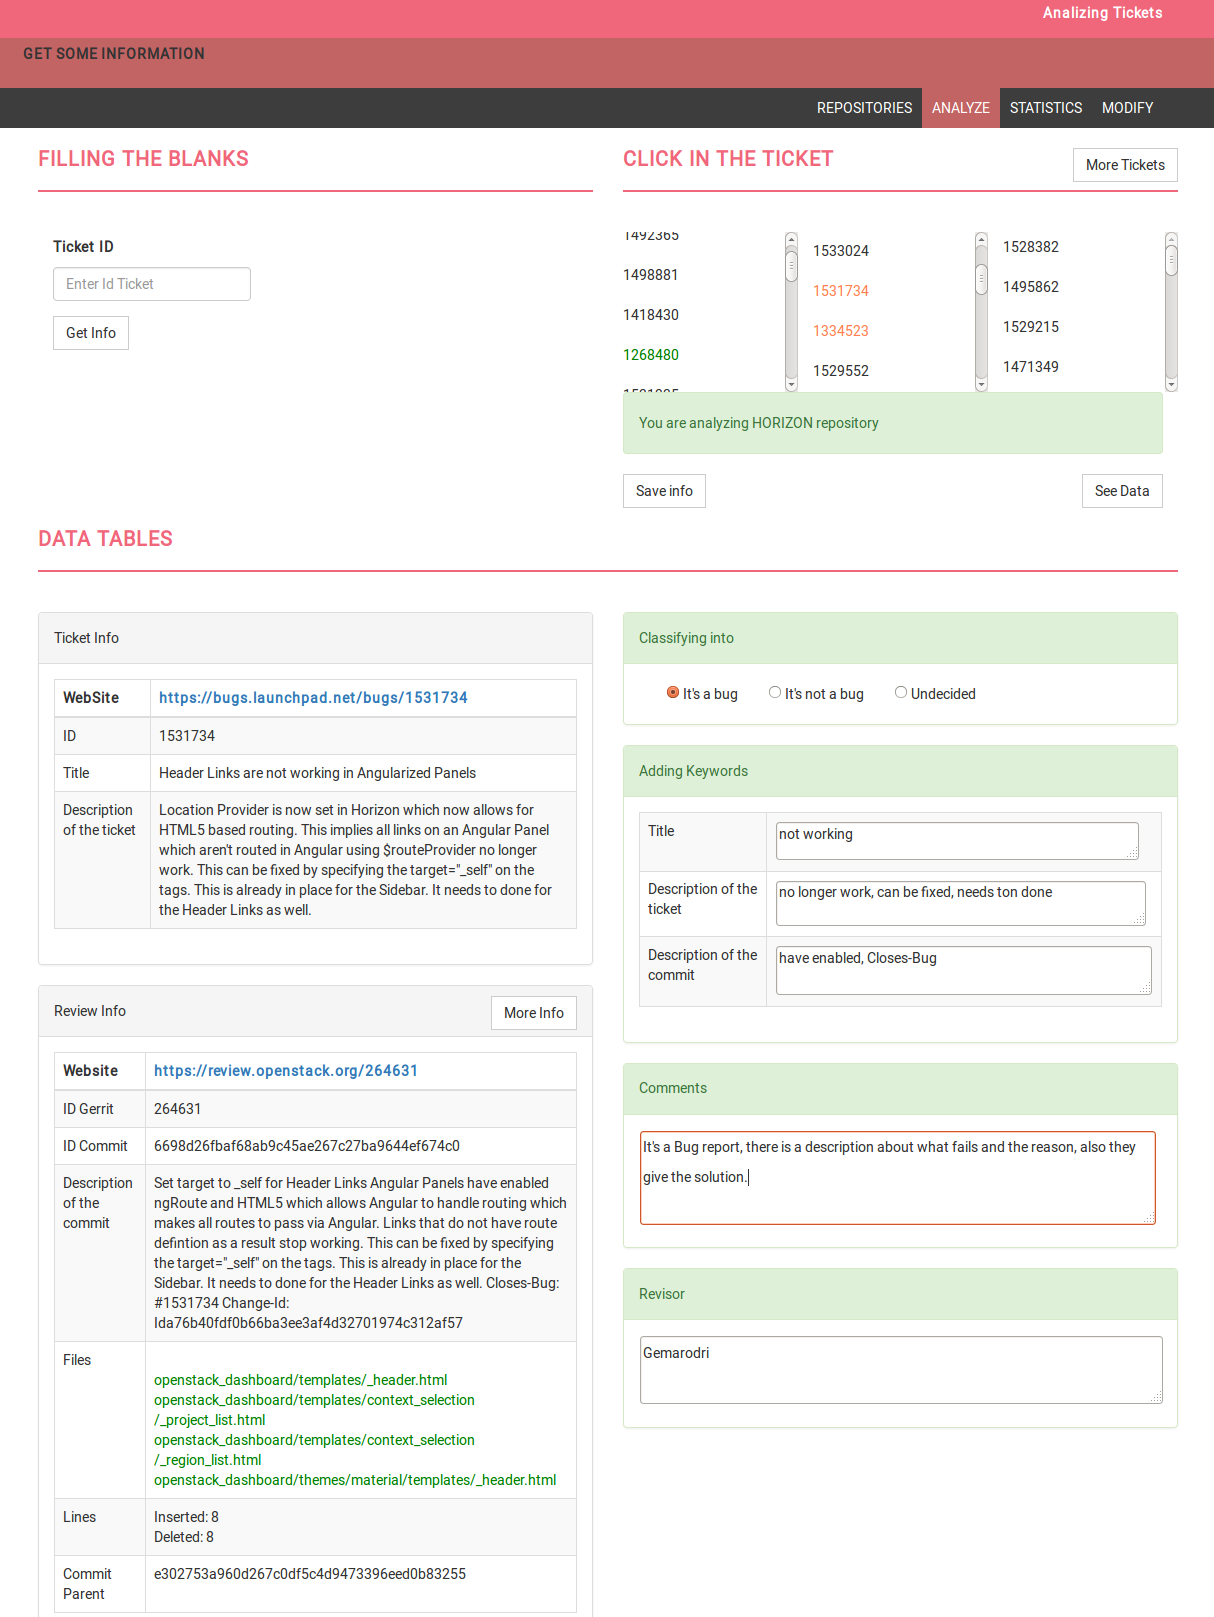
\includegraphics[height=15cm]{index.png}
\caption{Screenshot of Analyze Tab}
\label{fig:1}       % Give a unique label
\end{figure*}

\subsection{Second Stage: Responsability of Previous Commit}
\label{sec:secondStage}
In the second stage, we only focused on the analysis of \textit{Bug Report} group, because this group contained the tickets that we are sure were bug reports. Discarding the \textit{Undecided} group in favour of the \textit{Bug Report} group reduces the accuracy of the experiment due to the fact that some errors are being lost in \textit{Undecided} group. However the \textit{Undecided} group being only 6\% of the bugs under consideration makes us think that this fact does not affect the validity of the final results.

We focused on analyzing the previous commits involved in a bug fix, understanding previous commit as the last commit that touched the line that has been fixed in the bug fix commit. The image \ref{fig:2} shows a real example in which the commit 31f208423 injected the lines 715, 716 and 717 in the file. But in the line 716, this commit inserted a bug. According to the description of the commmit that fixed the bug, image \ref{fig:3}, the value in the variable of the line 716 had to be boolean, obtaining that the previous commit is responsible to cause the bug.
\begin{figure*}
\centering
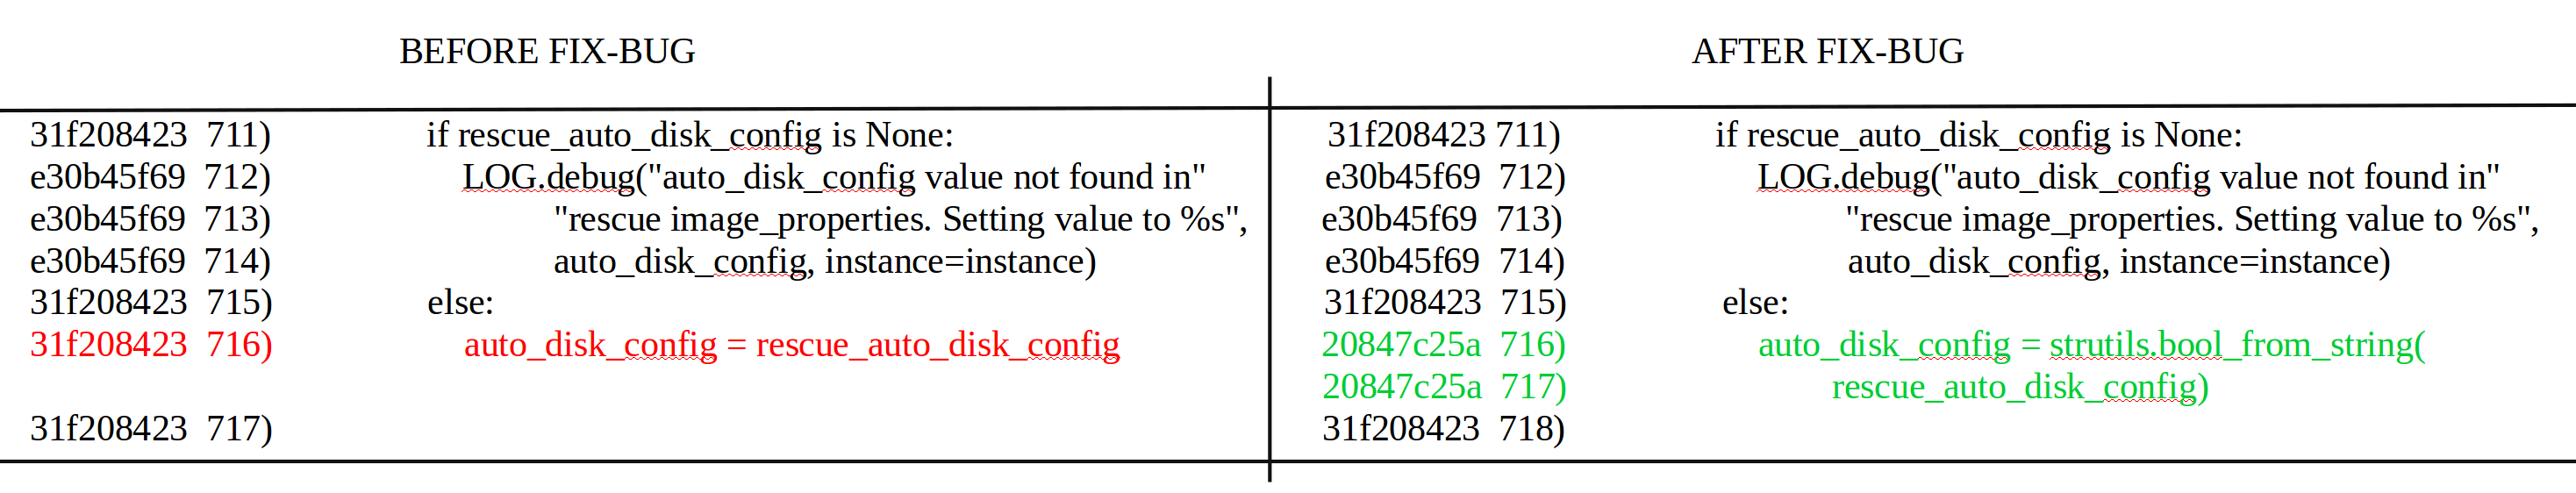
\includegraphics[height=2in, width=7in]{previouscommit.png}
\caption{Example of previous commit. The 31f208423 is the previous commit in the line involved in the bug-fix}
\label{fig:2}       % Give a unique label
\end{figure*}

\begin{figure}[htb]
\centering
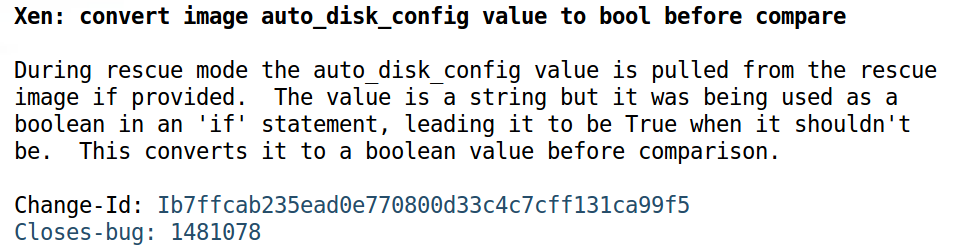
\includegraphics[height=2.3cm]{gerritPrevCommit.png}
\caption{Description of the bug-fix commit}
\label{fig:3}       % Give a unique label
\end{figure}


At this stage, we got a list with all the previous commits, which could be where the bug was introduced. We  identifyed a total of 348 previous commits which can be responsible for inserting the line with the bug. When there are more than one commit implicated in the same file is because the bug was inserted in different lines of different commits, but not everyone has to be responsible for the commit, sometimes the previous commit copied lines from its previous commit or inserted comments and blank spaces. After the analysis the responsible can be only one of them, more than one or none. 

We analyzed a total of 209 tickets in which there were 348 previous commit, which we had to classify into one of the following groups, according to the responsability of the previous commit in the bug fix:
\begin{enumerate}
  \item It is responsible, when we are sure that the commit inserted the line with the bug.
  \item It is not responsible, when we are sure that the commit dind't insert the line with the bug.
  \item Undecided, when we cannot be sure if the commit is responsible due to our few knowleadge about the project or when the bug fix only added lines, complicating the analysis.
\end{enumerate}

For that, we had to analyze the lines involved in the bug fix, in the commit parent of the bug fix commit, and to be sure that the lines was inserted/modified in the previous commit, we have to analyze these lines in the commit parent of the previous commit. This, way we can sure that the previous commit didn't copied any line that contained the bug, because in this case, the previous commit is not responsible to cause the bug. 

The analisys was done manually, and we used \textit{git blame} to see all the previos commit in each line of a involved file. In \ref{fig:4}, we can show the steps following to discover the responsible of the bug.
\begin{enumerate}
  \item git checkout \textit{commmit that fix the bug}, git blame \textit{file involved}. In this step we can see the lines added, modified or deleted by the commit that fix the bug.
  \item git checkout \textit{parent of commmit that fix the bug}, git blame \textit{file involved}. In this step we can see all the previous commits involved in the different lines touched in the fix bug.
  \item git checkout \textit{parent of previous commit}, git blame \textit{file involved}. In this step we can esure that the previous commit inserted these lines.
\end{enumerate}

\begin{figure*}[htb]
\centering
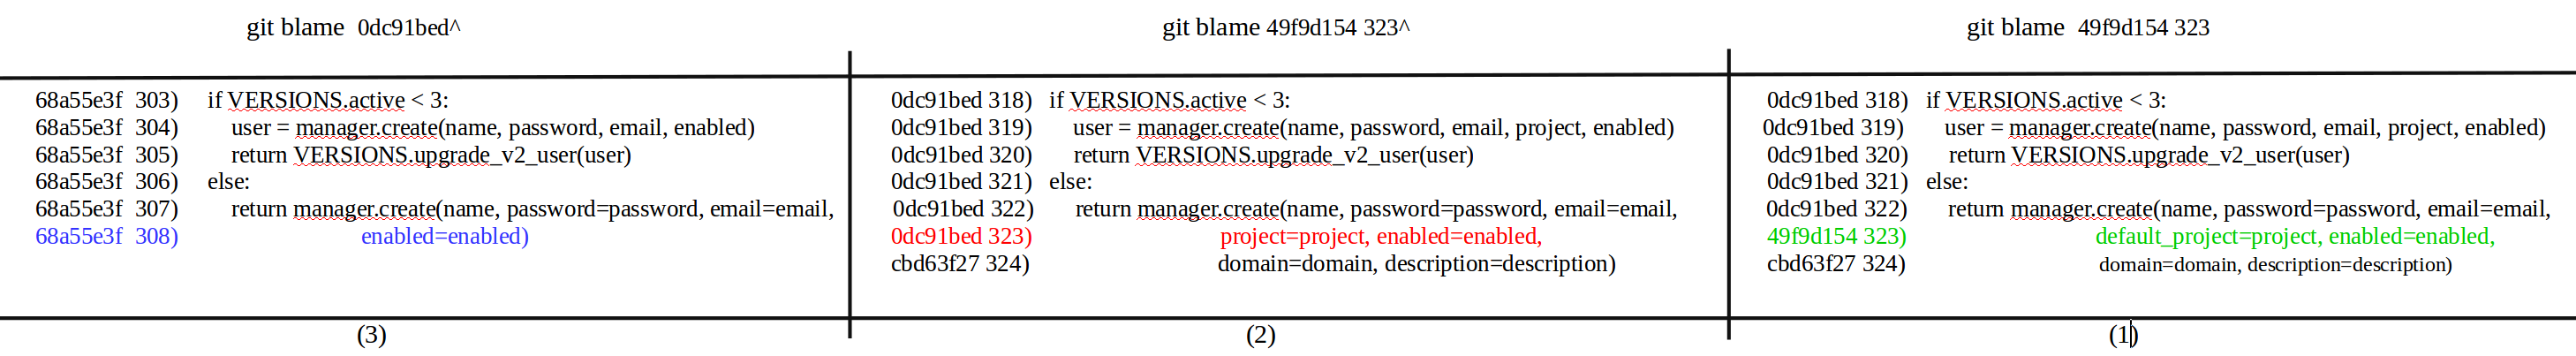
\includegraphics[height=2in, width=7in]{gitBlame.png}
\caption{Process to discover the commit that caused the bug }
\label{fig:4}       % Give a unique label
\end{figure*}

%To analyze the lines of the files involved, we used therefore the \texttt{diff} command to display line-by-line difference between the file before and after the bug fix commit. \texttt{diff} is well-known algorithm, extensively explained in the research literature~\cite{ukkonen1985algorithms,myers1986ano}, which is included in any source code management system. \texttt{diff} examines both files and returns the differences found between them, showing the line number.% the necessary modifications which should be done in order to the files match. the differences found between them,showing the line number. %FIXME: de aqui en adelante no entiendo la frase. need to be made for first file and second file to match, that is, returns the differences found between them.

After analayzed all the previous commit involved in the 209 Bug reports, we have discovered that not all the previous commits inserted the bug. This expecific project, which is continuosly evolving, presents some cases in which the bug was introduced by other actions. A clear example is the changes in called APIs, after the addition of a new feauture the called API fails, due to it requires an extra argument, but in the API there is not any bug.

Other example is shows in the commit log of a bug fix \ref{fig:5}, the name of a variable changed in the new version causing a failure. This change due to the new requirements in the version doesn't implicate that the previous commit was who inserted the bug, because until the new version the system doesn't fail.

\begin{figure}[htb]
\centering
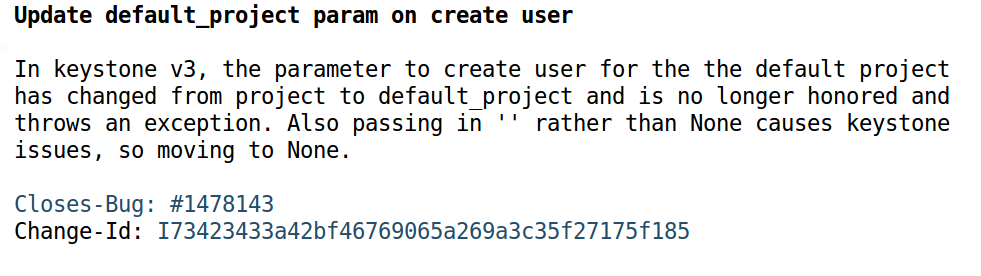
\includegraphics[height=2.3cm]{UpdateFixBug.png}
\caption{Description of the bug-fix commit}
\label{fig:5}       % Give a unique label
\end{figure}

\subsubsection{Discarting False Positives}
\label{sec:discarting}
The classification of the previous commits according to its responsability has some noise that we had to delete. These previous commits that changed the format, added blank lines, changed comments or copied lines from the previous commit were discarted due to they were not responsibles for cause the bug.


\section{Results}
\label{sec:results}

\subsection{Fist Stage}
\label{sec:resultsFS}
We have manually analyzed 459 different tickets with support of the present tool, 125 from Cinder, 125 fron Nova, 125 from Horizon and 84 from Neutron. The table \ref{tab:1} show the percentage of each researcher after analyzing the tickets, 417 tickets were analyzed by two different researchers, 

\begin{table*}
\centering
%\begin{center} {\footnotesize
\caption{ Classification statistics of each researcher}
\label{tab:1}
\begin{tabular}{lllll}
\toprule[0.3mm]%{\smallskip}
  & Bug Report\kern 1pc & Not Bug Report\kern 1pc & Undecided\kern 1pc & Total \\\hline
Researcher 1 \kern 1pc & (184) 55\% & (115) 34\% & (35) 11\% & 334 \\
Researcher 2 \kern 1pc & (188) 76\% & (54) 22 \% & (7) 3\% & 249 \\
Researcher 3 \kern 1pc & (188) 56\% & (116) 35\% & (30) 9\% & 334 \\
Total Concordance\kern 1pc & 209 & 74 & 6 & 292 \\
\bottomrule[0.3mm]
\end{tabular} %}
%\end{center}
\end{table*}

\subsection{Second Stage}
\label{sec:resultsSS}

\begin{table}[htb]
\begin{center} {\footnotesize
\caption{ Probability of cause the bug depending on how many previous commits had the bug report}
\label{secondStage}
\begin{tabular}{lcc}
\toprule[0.3mm]
  & \multicolumn{1}{c}{After} & \multicolumn{1}{c}{Before} \\
  & \multicolumn{1}{c}{False Negative} & \multicolumn{1}{c}{False Negative} \\\hline
\raisebox{1ex}{Responsible} & 152 & 152 \\[0ex]
\raisebox{1ex}{Not responsible} & 154 & 114 \\[0ex]
\raisebox{1ex}{Undecided} & 42 & 42 \\[0ex]
\bottomrule[0.3mm]
\end{tabular} }
\end{center}
\end{table}

58 tickets with more than one previous commit and 131 with only one previous commit
\begin{table}[htb]
\begin{center} {\footnotesize
\caption{ Probability of cause the bug depending on how many previous commits had the bug report}
\label{secondStage}
\begin{tabular}{lcc}
\toprule[0.3mm]
  & \multicolumn{1}{c}{One previous } & \multicolumn{1}{c}{More than one previous} \\
  & \multicolumn{1}{c}{commit} & \multicolumn{1}{c}{commit} \\\hline
\raisebox{1ex}{Responsible} & 65\% & 86\% \\[0ex]
\raisebox{1ex}{Not responsible} & 30\% & 82\%\\[0ex]
\raisebox{1ex}{Undecided} & 36\% & 11\%\\[0ex]
\bottomrule[0.3mm]
\end{tabular} }
\end{center}
\end{table}

\section{Discussion}
\label{sec:discussion}

This section presents first the threats to the validity of our study. Then, it discusses the possible applications and introduces the work that still has to be done. 

Once we have all the tickets analyzed by diferents researchers who have used a double blind, how to proceed if there are discordances between them:
\begin{enumerate}
\item Should they discuss after their analysis to reach a better classification?, Should the tool provide this?
\item Does the Bug report only the same ticket classified as Bug report for all the researchers?
\end{enumerate}

How to proceed if looking for the responsability of a bug when only added lines are inserted? And we are talking about a bug report not a new feature, these kinds of cases use to be when a researcher forgot check some case inside a function. [reference]
\begin{enumerate}
\item Is responsible the function where these lines are content?
\item Is responsible the last commit that modify something in the function?
\end{enumerate}


\section{Threats to validity}
\label{sec:threats}
The limited sample size of tickets used in this research is the major threat to its validity. %It may happen, that only with 100 seemingly random tickets, there may be a prior unknown tendency. This is in fact similar to~\cite{sliwerski2005changes}, where the trend indicates that most bugs are fixed on Fridays.

In addition our model has threats, external and internal, that make our model not 100\% valid. The internal threats are following:

\begin{itemize}
    \item We have not taken into account errors that have been classified into \textit{Undecided}.
    \item There could be some lax criteria involving the subjective opinion of the reviewers.
    \item We are not experts in analyzing and classifying tickets, and our inexperience may have influenced the results of the analysis.
    \item We are only using part of the information that the ticket provides, like comments and text. There could be a recognized pattern, unknown at first sight, that involves other parts of the information, or the whole information.
\end{itemize}

The external threats, related to the researchers that have conducted the classification, are following:

\begin{itemize}
    \item The word \textit{bug} is continuously mentioned in the description and commit of a ticket even when we found it is not an error. This could lead to the incorrect classification during the reviewing process.
    \item Some tickets are not explicitly described, which could increase the percentage of \textit{Undecided}. This is especially true if the reviewers are not from OpenStack.
\end{itemize}

\section{Related Work}
\label{sec:related}
First SZZ\\
Second Improvement of SZZ\\
Then SZZ revisited\\
Then Buginnings\\
Finally our idea.

\section{Conclusions}
\label{sec:conclusions}



%ACKNOWLEDGMENTS are optional
\section{Acknowledgments}
We thank the two phd students, Dorealda Dalipaj and Nelson Sekitoleko, that participated differentiating Bug report from the others. Also, we thank Bitergia \footnote{\url{http://bitergia.com/}} to explain its available database of OpenStack. 
Finally,thanks the Spanish Goverment because all authors are funded in part by it, through project TIN2014-59400-R.

\nocite{*}
%
% The following two commands are all you need in the
% initial runs of your .tex file to
% produce the bibliography for the citations in your paper.
\bibliographystyle{abbrv}
\bibliography{sigproc}  % sigproc.bib is the name of the Bibliography in this case
% You must have a proper ".bib" file
%  and remember to run:
% latex bibtex latex latex
% to resolve all references
%
% ACM needs 'a single self-contained file'!
%
%APPENDICES are optional
%\balancecolumns
\end{document}
